\clearpage
\section{Basics of Artificial Intelligence}
\label{sec:basics_artificial_intelligence}

\subsection{What is AI and Why Does It Matter Now}

\textbf{Artificial Intelligence} (AI) is the idea of making computers do things that normally need human thinking, like recognising objects in a picture, understanding language, or making decisions in complex situations \cite{goodfellow2016deep}. It is not one single technology but a big family of methods that all share the same goal: teach machines to learn from data and improve over time.

\begin{figure}[H]
\centering
\setlength{\fboxsep}{4pt}
	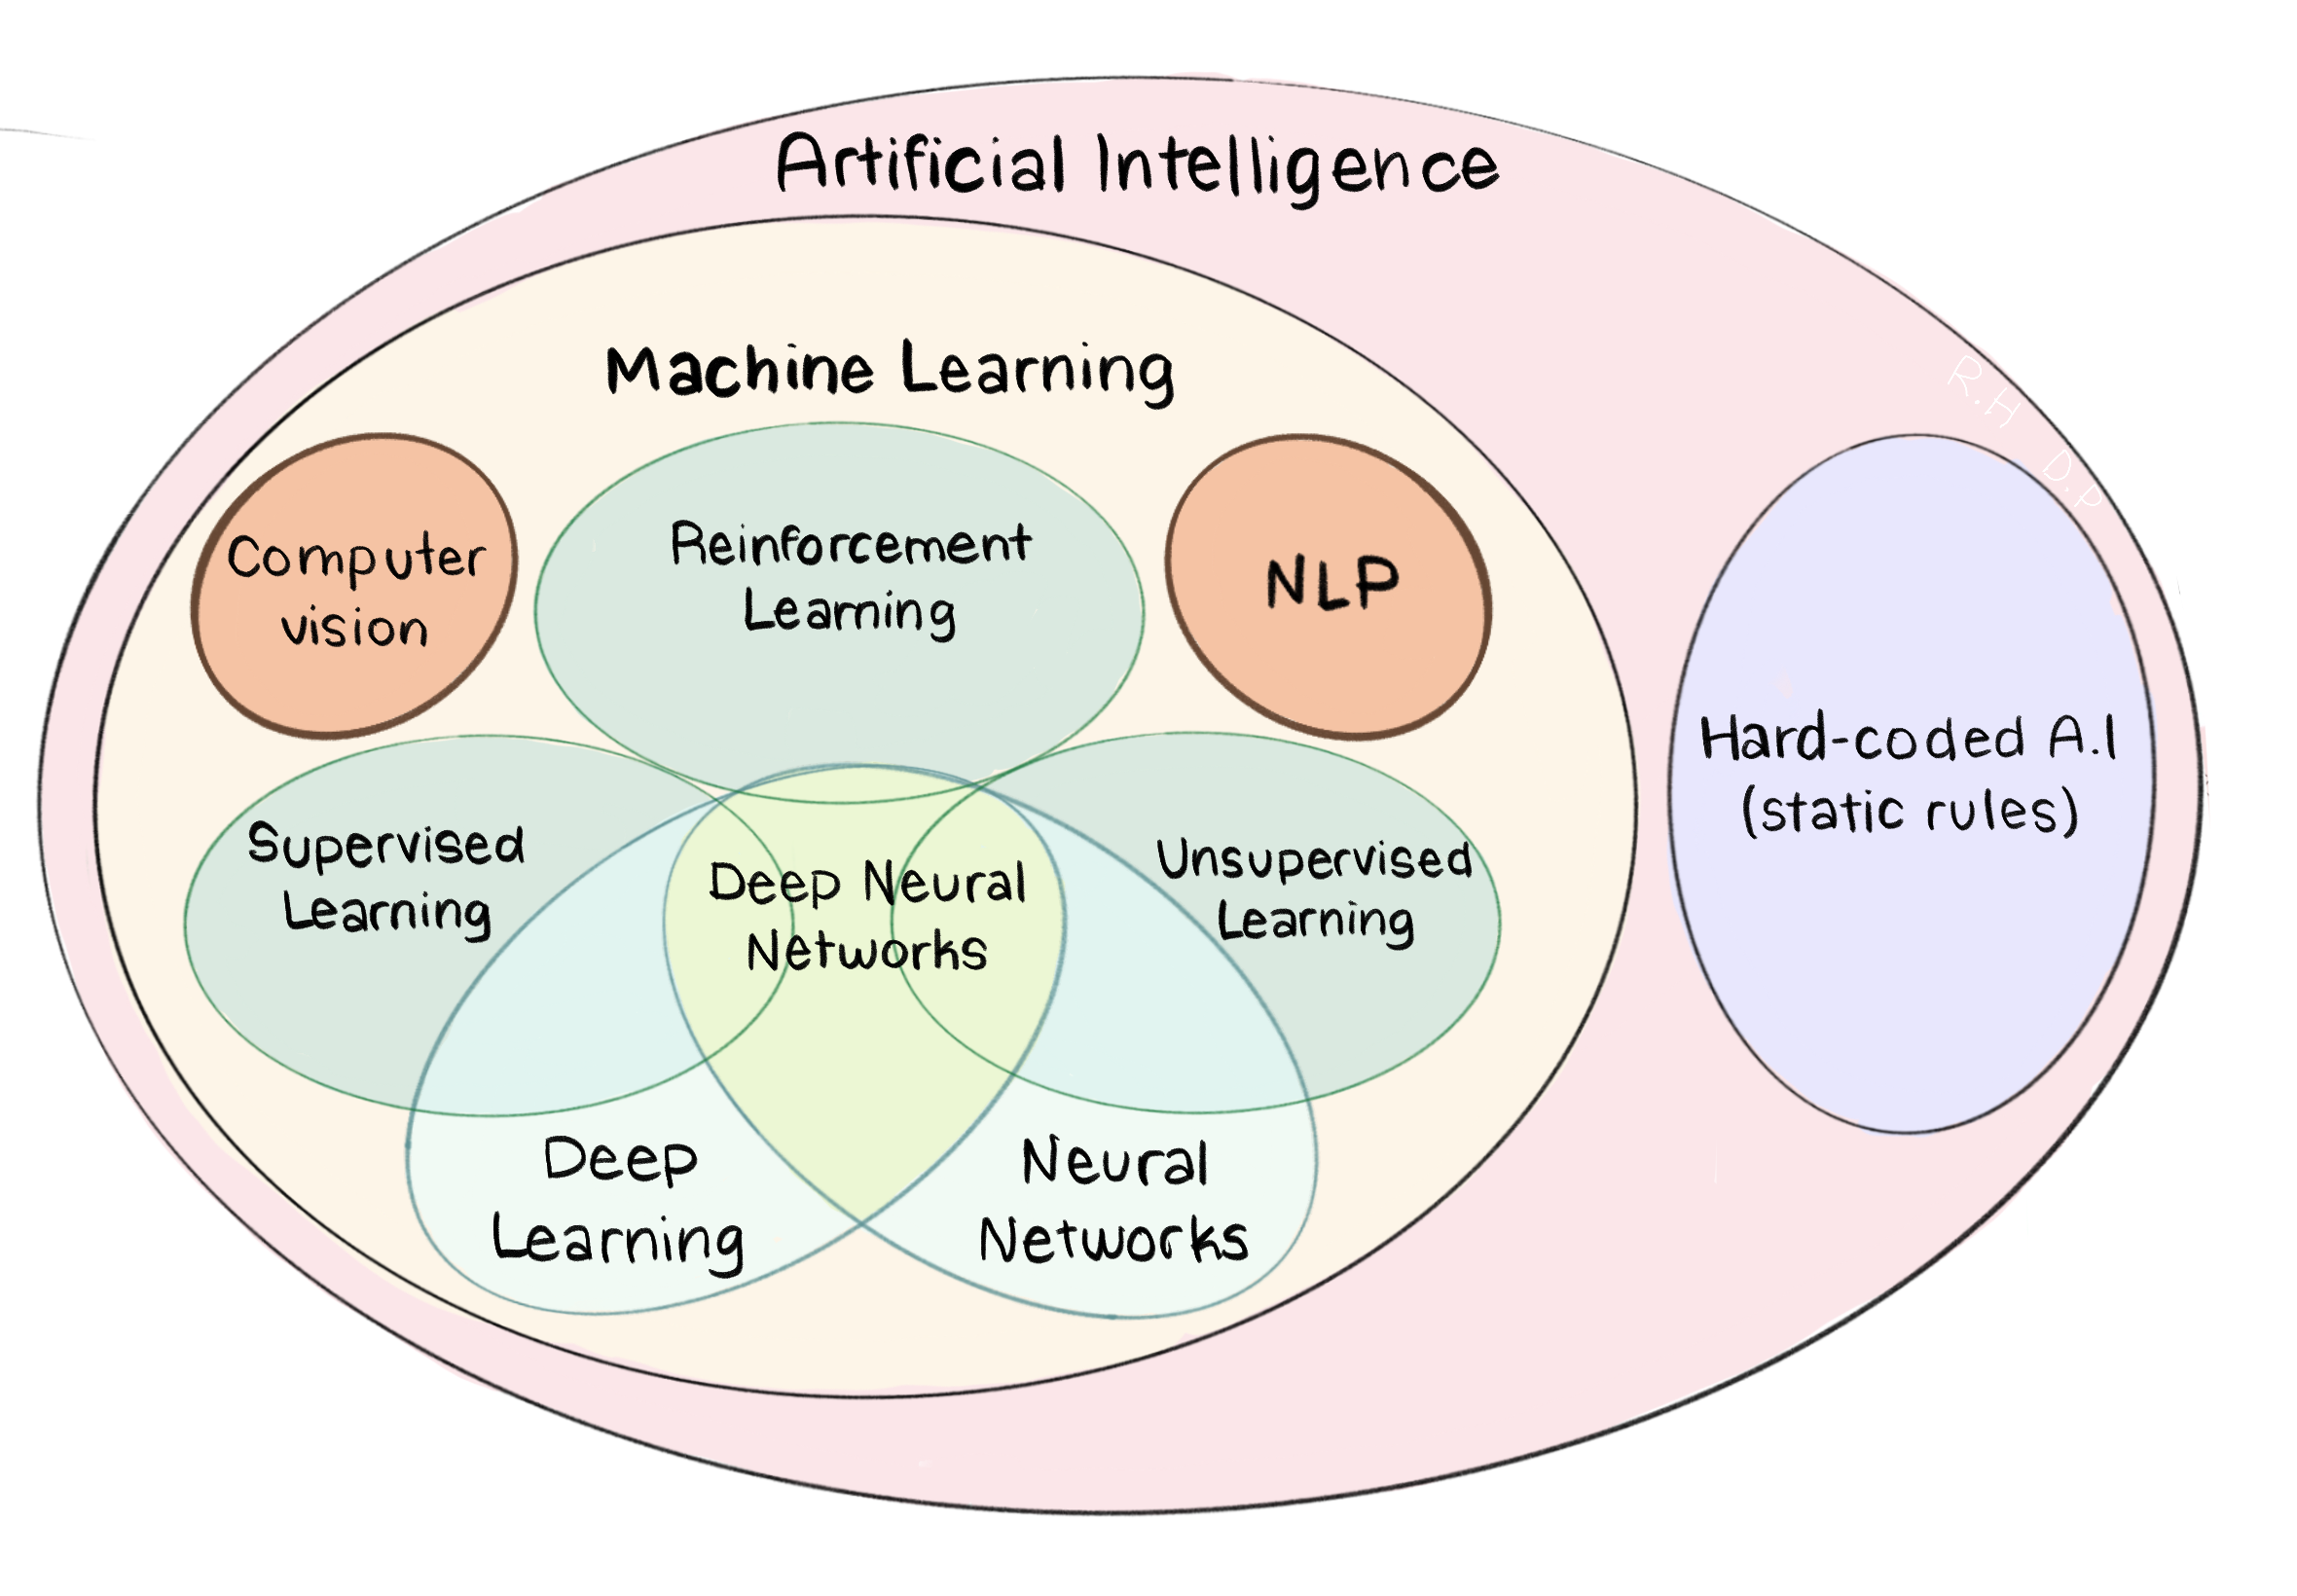
\includegraphics[width=1\linewidth]{assets/diagram-a.i-venn.png}%
\caption{How the main fields of AI relate to each other.}
\label{fig:ai_venn}
\end{figure}

The field has been around since the 1950s, but it really took off in the last decade thanks to three things happening at the same time: much bigger \textbf{datasets}, much faster \textbf{hardware} (especially GPUs), and better \textbf{algorithms} like deep neural networks \cite{litjens2017dlSurvey}. To give an idea of how fast things are moving, the famous \textbf{AlphaGo} system by DeepMind beat the world champion in the board game Go in 2016, a task that many researchers thought was still decades away \cite{silver2016alphago}. That moment really showed the world what modern AI could do.

Inside the AI family, there are a few important subfields that we use in this project:

\begin{itemize}
\item \textbf{Machine Learning (ML):} methods that let a computer learn patterns from data without being told exactly what to look for.
\item \textbf{Deep Learning (DL):} a part of ML that uses neural networks with many layers, and it is especially good at working with images and video.
\item \textbf{Computer Vision (CV):} techniques for understanding what is in an image or a video, like detecting objects or tracking motion.
\item \textbf{Deep Reinforcement Learning (Deep RL):} a way for an agent to learn by trying actions and getting feedback (rewards or penalties) from the environment.
\end{itemize}



What makes AI so exciting right now is that these subfields are starting to work together. In our project, for example, we use deep learning to understand what the camera sees (that is the computer vision part), and then deep reinforcement learning to decide what to do next. This combination is what makes intelligent agents possible.

\subsection{How AI is Already Used in Medicine and Endoscopy}

AI is not just a research topic anymore. It is already being used in real hospitals. In radiology, AI systems help doctors read X-rays and CT scans faster. In pathology, they help analyse tissue samples. And in \textbf{endoscopy}, which is the field that interests us most, AI is making a real difference.

One of the most exciting results in recent years came from clinical trials that tested \textbf{computer-aided detection} (CADe) systems during colonoscopy. These systems run in real time and highlight suspicious areas on the screen to help the doctor spot polyps. A large randomised trial by Wang et al. found that using a CADe system increased the \textbf{adenoma detection rate} from \textbf{20\,\%} to \textbf{29\,\%}, which is a big improvement \cite{wang2019cade}. Another trial by Repici et al. confirmed similar results, showing that AI-assisted colonoscopy finds more polyps without making the procedure longer \cite{repici2020cade}.

These systems are mostly focused on \textbf{detection}, meaning they help the doctor see the polyp. But the next big question is: can AI also help with the \textbf{treatment} itself? That is where our project comes in.

A good survey by Nazarian et al. looked at many studies on AI for polyp detection and characterisation, and found that deep learning models can reach a \textbf{sensitivity above 90\,\%} in detecting colorectal polyps from endoscopic images \cite{nazarian2021jmir}. That means the technology is already quite reliable for spotting lesions. But actually removing them safely is a very different challenge.

\subsection{What Our Agent Needs to Do: Navigate and Extract}

In this project, we are not building a polyp detector. Instead, we are building an agent that can \textbf{act} inside a simulated colon. The agent has two main jobs:

\begin{itemize}
\item \textbf{Navigate:} the agent must guide the endoscope tip through the colon, avoid hitting the walls, keep a clear view, and reach the area where the polyp is located. This is like driving through a narrow, winding tunnel where the walls are soft and the lighting keeps changing.
\item \textbf{Extract:} once the agent is close enough to the polyp, it needs to use a snare tool to grab and remove it. This means extending the snare, positioning it around the polyp, and closing it at the right moment without damaging the surrounding tissue.
\end{itemize}

Both tasks are \textbf{sequential}, which means each action affects what happens next. A bad move now can make the next step much harder. That is exactly the kind of problem where deep reinforcement learning works well, because the agent learns to think ahead and not just react to the current frame.

The agent uses a \textbf{CNN} to understand what the camera sees, an \textbf{LSTM} to remember what happened a few steps ago, and \textbf{PPO} (a deep reinforcement learning algorithm) to decide what to do next. We will explain each of these in the following sections, starting with deep reinforcement learning.
